% !TeX root = main.tex


\begin{savequote}[70mm]
,,''
\qauthor{}
\end{savequote}


\chapter{Aplikacje i testy}
\label{chap:aplikacje}

\section{Automatyczna kalibracja odometrii i żyroskopu}

Proces kalibracji odometrii oraz pomiarów uzyskiwanych z żyroskopu został
przestawiony w rozdziale~\ref{chap:software}. W celu jego ułatwienia i
zautomatyzowania stworzona została aplikacja przeprowadzająca dwuetapową
kalibrację -- najpierw wyliczająca poprawki dla współczynników kątowych
żyroskopu i odometrii, a następnie licząca poprawkę dla składnika liniowego
odometrii. Aby poprawnie przeprowadzić cały proces wymagana jest pusta
przestrzeń o powierzchni ok. 2x2m, oraz płaska powierzchnia na jednym z końców
(np. ściana).

\subsection{Wyznaczanie odległości i kąta obrotu względem ściany}

W celu wyznaczenia faktycznej wartości obrotu wykonanego przez robota oraz
określenia pokonanej odległości, wymagana jest obecność sensora zwracającego
odczyty laserowe (w przypadku robota Elektron możliwe jest wykorzystanie
zarówno skanera SICK jak i sensora Kinect z dodatkowym komponentem
zamieniającym pomiary z chmury punktów na symulację odczytu laserowego). Na
podstawie punktów zwracanych przez sensor ustawiony na przeciwko ściany
wyliczana jest orientacja robota względem niej, a także odległość.

\subsubsection{Orientacja}

Dane odczytane z lasera mają postać zbioru punktów we współrzędnych biegunowych.
Pierwszym krokiem jest ich przeliczenie na współrzędne kartezjańskie w układzie
związanym ze środkiem sensora. Po takim przeliczeniu, wykorzystując metodę
najmniejszych kwadratów, wyliczane są parametry prostej przechodzącej możliwie
blisko danych punktów. Współczynnik kierunkowy tej prostej określa jednocześnie
orientację robota względem ściany.

Mając dane punkty w postaci $(x_i, y_i)$, gdzie $i=1\ldots n$, oraz przyjmując
oznaczenia:

\[
S_x = \sum_{i=1}^n x_i \mathsp
S_y = \sum_{i=1}^n y_i \mathsp
S_{xx} = \sum_{i=1}^n x_i^2 \mathsp
S_{xy} = \sum_{i=1}^n x_i \cdot y_i \mathsp
%S_{yy} = \sum_{i=1}^n y_i^2 \mathsp
\Delta = n \cdot S_{xx} - S_x^2
\]

Współczynniki prostej o równaniu $y=a\cdot x+b$ wyznaczane są przez wzory:

\[
a = \frac{n \cdot S_{xy} - S_x \cdot S_y}{\Delta} \mathsp
b = \frac{S_{xx} \cdot S_y - S_x \cdot S_{xy}}{\Delta}
\]

Skąd orientację robota względem ściany (wyznaczonej prostej) uzyskujemy ze
wzoru:

\[
\phi=atan(a)
\]

\subsubsection{Odległość}

Wykorzystując już punkty we współrzędnych kartezjańskich, odległość od ściany
wyliczana jest jako średnia z wartości $y$ wszystkich punktów.

\subsection{Właściwy proces kalibracji}

Przed rozpoczęciem kalibracji robot powinien zostać ustawiony na wprost ściany,
w odległości ok. 50cm od niej. Pierwszą czynnością po uruchomieniu zadania jest
wyznaczenie składowej stałej pomiarów z żyroskopu, po czym następują trzy
pełne obroty robota z różnymi prędkościami (fakt wykonania pełnego obrotu
wyznaczany jest na podstawie odczytów z odometrii). Po wykonaniu każdego obrotu
wyliczana jest faktyczna jego wartość (na podstawie porównania orientacji
względem ściany zmierzonej przed i po wykonaniu obrotu), a razem z nią
zapamiętywane są wartości obrotu odczytane z odometrii i żyroskopu. Pomiędzy
kolejnymi pomiarami robot jest pozycjonowany powtórnie na wprost ściany (z
pewną, niewielką tolerancją) wykorzystując pomiary laserowe. Po wykonaniu
wszystkich obrotów wyliczane są błędy wskazań odometrii i żyroskopu (stosunek
wartości odczytanej do zmierzonej laserem), a z nich wyliczana jest średnia
wartość poprawki, którą należy wprowadzić do współczynników obrotowych obu
badanych czujników.

Po wykonaniu kalibracji obrotów robot powtórnie ustawia się na wprost ściany, a
następnie odjeżdża od niej na odległość ok. 2 metrów. Następnie przejeżdża 1.5
metra do przodu, a po przejechaniu tego dystansu wyliczana jest poprawka
współczynnika liniowego odometrii (stosunek przejechanej odległości wyliczonej
przez odometrię do odległości uzyskanej z pomiarów laserowych). Ostateczna
wartość poprawki wyliczana jest jako średnia z trzech takich przejazdów z
różnymi prędkościami. Uzyskane w tym procesie wartości współczynników należy
pomnożyć przez współczynniki już ustawione w sterownikach robota.



\section{Prosta, losowa eksploracja}

Kolejną aplikacją, która powstała w celu przetestowania porawnego działania
sensorów oraz sterownika silników była losowa eksploracja terenu. Podczas
ruchu wyznaczana jest minimalna odległość do przeszkód w dwóch strefach
-- po lewej oraz prawej stronie. Jeśli wokół robota nie ma przeszkód bliżej,
niż ustalona odległość minimalna, to porusza się on na wprost. W przeciwnym
wypadku prędkość kątowa jest proporcjonalna do różnicy odległości przeszkód
po lewej i prawej stronie (o kierunku takim, aby dążyć do wyrównania odległości
po obu stronach), a prędkość liniowa proporcjonalna jest do średniej odległości
przeszkód po obu stronach.

Zadanie spełnia swoją podstawową rolę -- pozwala na przetestowanie różnych
zestawów sensorycznych (skanera laserowego, Kinecta) oraz zweryfikować
poprawność działania układu zarządzającego pracą silników. Niestety, ze względu
na bardzo prosty algorytm zastosowany do omijania przeszkód, zdarzają się sytuacje
blokady robota w narożnikach pomieszczeń (średnia odległość od przeszkód po
obu stronach jest taka sama, więc robot nie skręca, a ściany są na tyle blisko,
że prędkość liniowa została wyzerowana). Innym pojawiającym się problemem
jest wjeżdżanie w przeszkody podczas zakręcania przy korzystaniu z sensorów
o dużej minimalnej odległości działania i wąskim polu widzenia. Spowodowane jest
to brakiem jakiejkolwiek pamięci co do przeszkód (np. małej lokalnej mapy zajętości),
przez co jeśli robot stoi obok ściany (której nie wykrywa czujnikami, bo nie jest
w ich polu widzenia) i odwróci się w jej stronę, to moze na nią wjechać (czujniki
nie wykryją przeszkody, gdyż znajduje się ona zbyt blisko).



%\section{Budowa mapy}



\section{Dojazd do wyznaczonego celu z omijaniem przeszkód}

Ostatnią, a zarazem kluczową aplikacją stworzoną w ramach tej pracy jest
pełny system nawigacji (o strukturze opisanej w poprzednich rozdziałach)
przygotowany do możliwie maksymalnego wykorzystania wszystkich dostępnych
elementów (tj. układów sensorycznych, systemów lokalizacji). Eksperymenty
przeprowadzane były w laboratorium robotyki i jego okolicach, a więc w pomieszczeniach
o charakterze biurowo-warsztatowym, z wieloma obiektami przenoszonymi z miejsca
na miejsce. Szczególnie często na korytarzu zmieniała się konfiguracja przeszkód
-- przestawiane krzesła, drzwi otwierane czasami częściowo, czasami całkowicie,
a także przechodzący ludzie. Zgodnie z założeniami zadania, robot miał poradzić
sobie w takim srodowisku i dążyć do osiągnięcia zadanego celu.

\subsection{Scenariusz pracy}

Scenariusz działań podczas korzystania z tej aplikacji jest dość prosty -- początkowo,
po uruchomieniu robota i wszystkich niezbędnych modułów opisanych wcześniej, należy
wskazać jego przybliżoną pozycję i orientację na mapie. Następnym krokiem jest
wskazanie punktu docelowego, który robot ma osiągnąć. W zależności od jego osiągalności,
a w zasadzie tego, czy planer globalny będzie w stanie wyznaczyć prawidłowy plan
czy nie, podejmowane są różne akcje. Jeśli plan nie zostanie odnaleziony, to wyświetlany
jest odpowiedni komunikat oraz emitowany dźwięk oznaczający niepowodzenie wykonania
zadania. Jeśli ścieżka zostanie wyznaczona, emitowany jest dźwięk akceptacji celu
i rozpoczyna się wykonanie trajektorii, segment po segmencie. Podczas jazdy może się
okazać, że wyznaczona ściezka jest niemożliwa do wykonania (np. zostały zamknięte
drzwi, przez które wiodła trajektoria), robot się zatrzymuje i uruchamiany jest
ponownie planer globalny (z dodatkową wiedzą o stanie przeszkód w okolicy robota).
Po dojechaniu do wyznaczonego celu (z pewną, określaną z góry dokładnością zarówno
co do połozenia jak i orientacji) robot zatrzymuje się i emitowana jest informacja
o poprawnym wykonaniu zadania.

\subsection{Obsługa sytuacji wyjątkowych}

Odrębną sytuacją jest próba wybrnięcia z sytuacji wyjątkowych, w których mógł się
znaleźć robot. Do sytuacji takich należy przede wszystkim okrążenie przeszkodami.
Jest to stosunkowo częsta sytuacja, szczególnie że czujniki na robocie nie rejestrują
pełnego otoczenia, a jedynie jego fragment przed robotem oraz ewentualnie po bokach.
Jeśli przed robotem stanie człowiek, robot się odwróci, a obraz przeszkody pozostanie
na jego lokalnej mapie zajętości. Jeśli w ten sposób robot zostanie na chwilę okrążony,
to pomimo faktycznego zniknięcia tych obiektów, stanowią one przeszkodę dla algorytmu
wyznaczania ściezki lokalnej i sygnalizuje on zakleszczenie. W tym momencie uruchamiane
są zachowania mające na celu wyprowadzenie robota z tego stanu i oczyszczenie mapy
zajętości.

W przygotowanym systemie sterowania zachowania te są możliwe do łatwej zmiany, pozwalając
na eksperymenty z różneg rodzaju mniej i bardzej agresywnymi podejściami. W stworzonej
aplikacji wykorzystane zostały dwa domyślne podejścia. Pierwsze z nich po zatrzymaniu
robota czyści przeszkody znajdujące się dalej niż ustalony limit od robota. Drugie
wykonuje obrót w miejscu o 360\textdegree~wypełniając mapę aktualnymi informacjami
o środowisku wokół. Po uruchomieniu każdego z zachowań ratunkowych sprawdzane jest,
czy możliwe jest kontunyowanie jazdy, w przeciwnym wypadku uruchamiane jest kolejne
zachowanie, aż do wyczerpania wszystkich dostepnych możliwości. W takim wypadku
emitowana jest informacja o niepowodzeniu zadania. Graf rpzedstawiający kolejność
uruchamiania zachowań ratunkowych przedstawiony jest na rysunku~\ref{fig:recovery}.

\begin{figure}[h!]
\centering
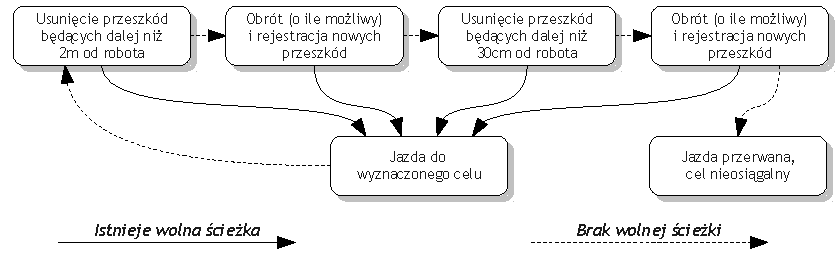
\includegraphics[width=\textwidth]{../img/recovery}
\caption{Zachowania ratunkowe}
\label{fig:recovery}
\end{figure}

\subsection{Weryfikacja poprawności działania}

Największym problemem w aplikacjach robotycznych jest weryfikacja poprawności ich
działania. Możliwe jest napisanie testów jednostkowych samego oprogramowania,
nie da się jednak stworzyć podobnych testów dla aplikacji wykorzystujących sprzęt
taki jak roboty. Istnieje kilka podejść przeprowadzania testów mających na celu
zwiększenie prawdopodobieństwa działania aplikacji zgodnie z oczekiwaniami.
Pierwszą metodą jest wykorzystanie symulatorów (zarówno ogólnodostępnych, jak
i specjalizowanych przygotowywanych specjalnie dla jednego robota). Kolejnym sposobem
jest przetestowanie aplikacji z wykorzystaniem właściwego robota w kontrolowanych
warunkach (z zachowaniem odpowiednich środków ostrożnośći). Istotne jest to, że
obie te metody można wykorzystać jednocześnie, sprawdzając najpierw ogólną poprawność
algorytmu na symulacji, a następnie sprawdzając wszystkie możliwe przypadki użycia
(a przynajmniej tyle, ile można przewidzieć).

\subsubsection{Wykorzystanie symulacji}



\subsubsection{Testy w kontrolowanych warunkach}


